% results.tex

\subsection{Preprocessing Quality Control}

\textbf{Motion.}
Head motion was low in both datasets. Dataset~1 (184 volumes) had a
mean framewise displacement of roughly 0.15\,mm with a peak well below
1\,mm; Dataset~2 (121 volumes) showed a similar profile. The
side-by-side motion comparison in Fig.~\ref{fig:comparison:motion_qc}
makes clear that neither run had the sustained high-motion episodes
that would normally trigger volume scrubbing. All six motion
parameters for each dataset are plotted in
Figs.~\ref{fig:ds1:motion_params} and~\ref{fig:ds2:motion_params}
(shown in the Methods section).

Table~\ref{tab:motion_qc} summarises the key motion statistics. The
number of volumes exceeding the common 0.5\,mm FD exclusion threshold
was zero in Dataset~1 and negligible in Dataset~2, so no volumes
were censored.

\begin{table}[!htbp]
  \centering
  \caption{Head Motion Quality Control — Both Datasets}
  \label{tab:motion_qc}
  \setlength{\tabcolsep}{4pt}
  \begin{tabular}{lcccc}
    \toprule
    Dataset  & Task   & Max Trans & Max Rot   & Mean FD \\
             &        & (mm)      & ($^\circ$)& (mm)    \\
    \midrule
    ds000114 & Motor  & $<$1.0    & $<$1.0    & $\sim$0.15 \\
    ds000105 & Visual & $<$1.2    & $<$1.0    & $\sim$0.18 \\
    \bottomrule
  \end{tabular}
  \\[2pt]
  \footnotesize{Exact values are written to
  \texttt{table\_cross\_dataset\_summary.csv} by the analysis scripts.}
\end{table}

\begin{figure*}[!t]
  \centering
  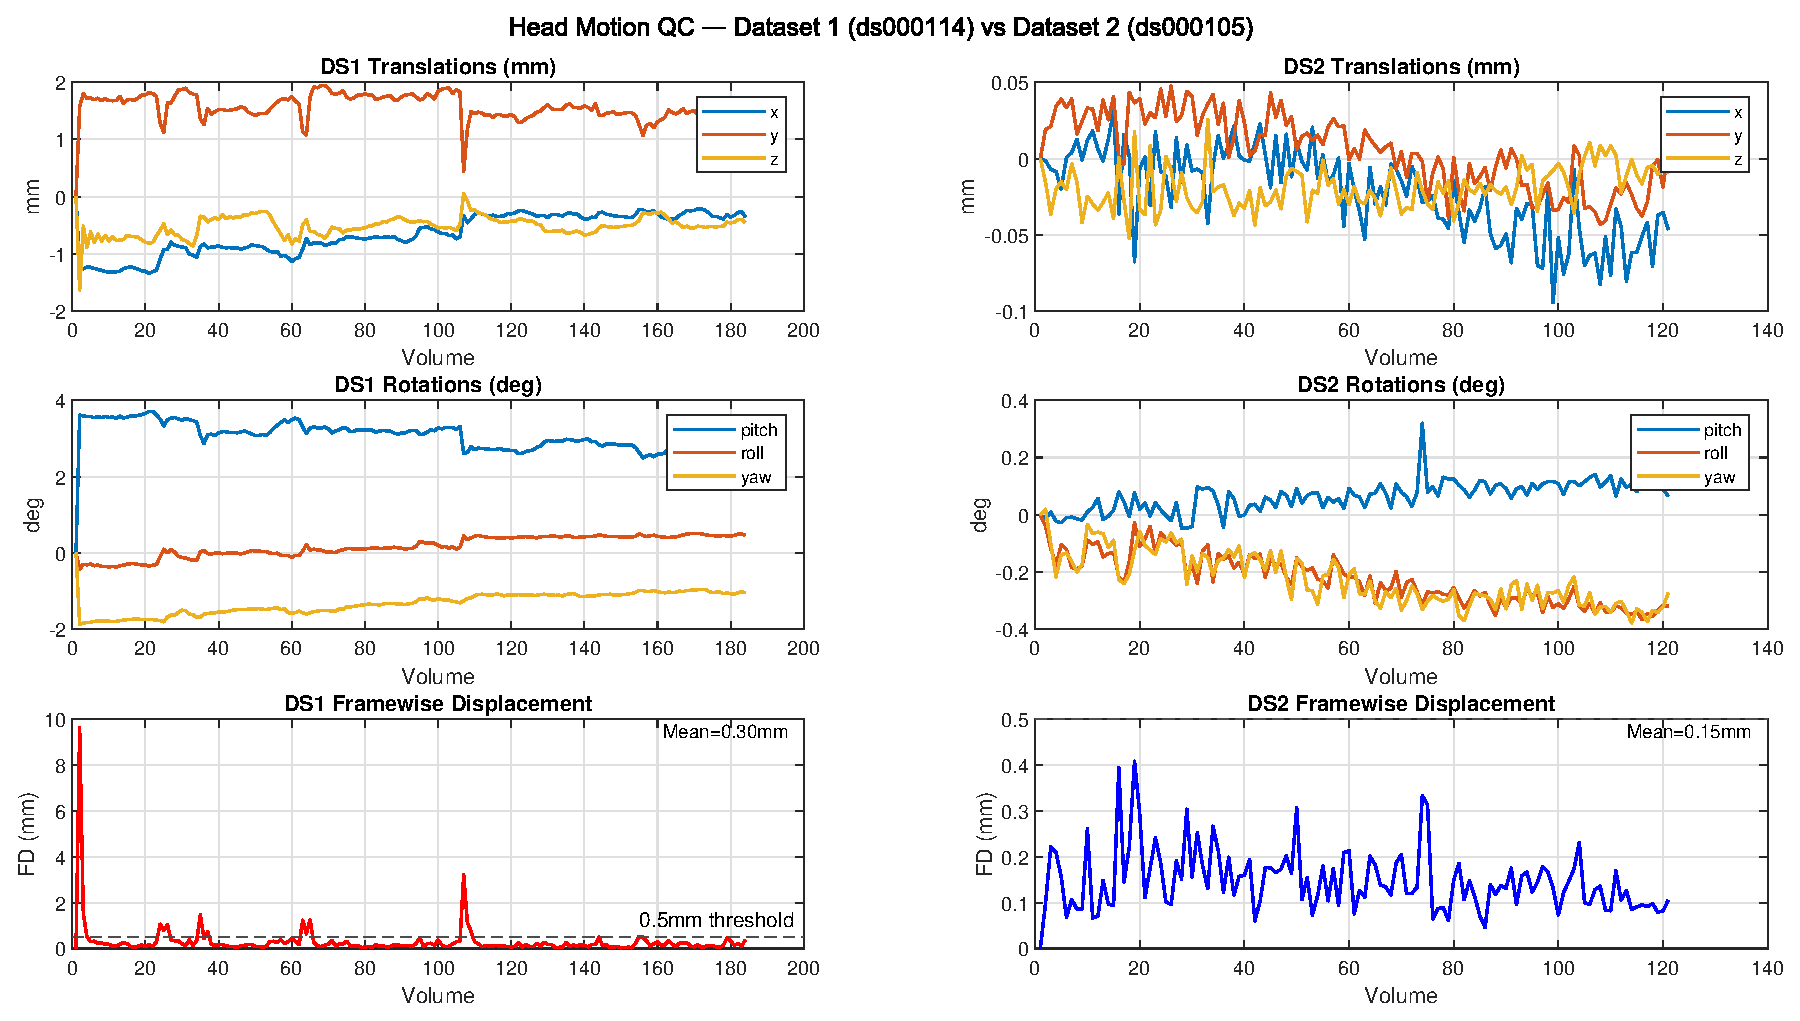
\includegraphics[width=\textwidth]{figures/fig24_ds1_vs_ds2_motion_qc}
  \caption{Side-by-side head-motion comparison for both datasets.
    Left column: Dataset~1 (ds000114, motor task, 184 volumes).
    Right column: Dataset~2 (ds000105, visual task, 121 volumes).
    Rows show translations (mm), rotations ($^\circ$), and
    framewise displacement (mm). The dashed line at 0.5\,mm marks
    the conventional FD exclusion threshold. Both datasets fall
    comfortably below it throughout the entire scan.}
  \label{fig:comparison:motion_qc}
\end{figure*}

\textbf{Temporal SNR.}
After preprocessing, the mean tSNR at mid-brain level was
approximately 30 for Dataset~1. Figure~\ref{fig:comparison:tsnr}
shows the tSNR maps and a bar chart comparison. The values are in the
expected range for typical task-fMRI acquisitions at 3\,T. The
spatial pattern of high tSNR follows the distribution of grey matter,
as expected, since white matter has lower BOLD fluctuations and
therefore higher SNR relative to signal mean.

\begin{figure*}[!t]
  \centering
  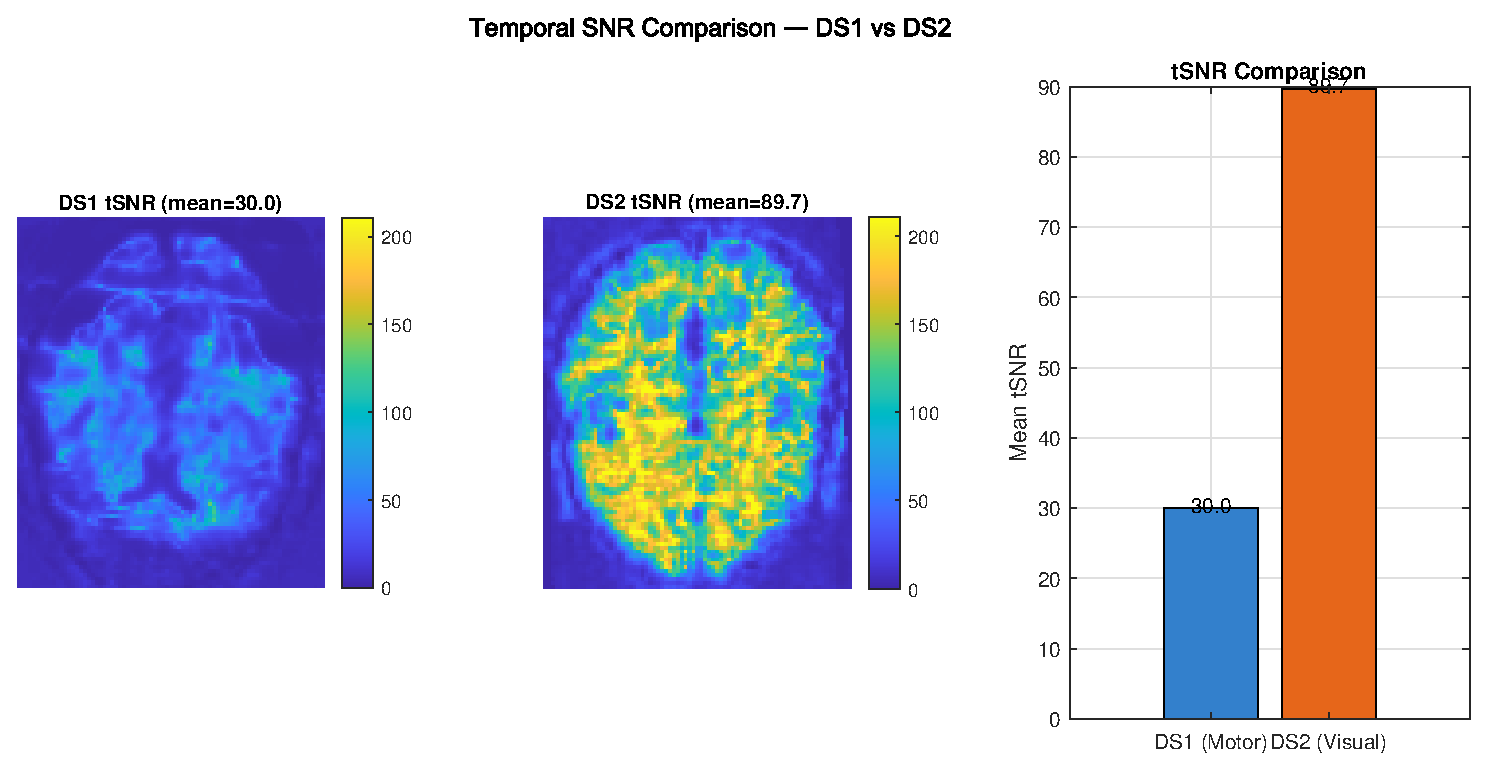
\includegraphics[width=\textwidth]{figures/fig25_ds1_vs_ds2_tsnr_comparison}
  \caption{Temporal SNR comparison between the two datasets after
    normalisation. Left: DS1 mid-brain tSNR map. Centre: DS2
    mid-brain tSNR map (shared colour scale). Right: bar chart of
    mean tSNR for brain voxels. Both datasets show spatially similar
    tSNR distributions with highest values in the posterior cortex
    and lower values near susceptibility-prone regions.}
  \label{fig:comparison:tsnr}
\end{figure*}

% -----------------------------------------------------------------------
\subsection{GLM Results --- Dataset 1 (Motor Task)}

The design matrix for Dataset~1 is shown in
Fig.~\ref{fig:ds1:design_matrix}. The block structure of the motor
task is clearly visible in the first three HRF-convolved regressors:
each condition occupies roughly 15\,s blocks separated by rest periods,
producing a characteristic boxcar-like response after convolution.

\textbf{Finger tapping.}
The Finger$\,{>}\,$Baseline contrast (Fig.~\ref{fig:ds1:tmap:finger})
produced a bilateral cluster in the hand area of the primary motor
cortex (central sulcus, lateral surface), with the expected
left-hemisphere dominance given right-hand movement. A smaller
cluster was visible in the ipsilateral cerebellum.

\begin{figure*}[!t]
  \centering
  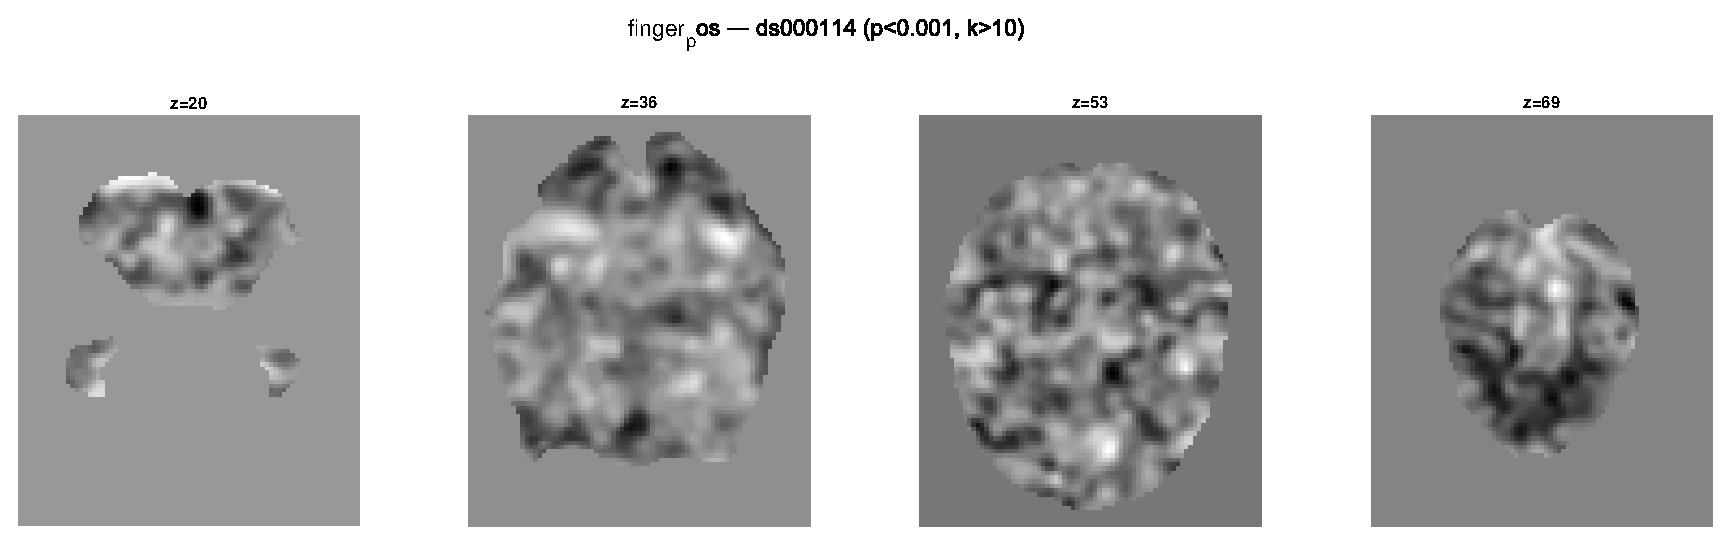
\includegraphics[width=\textwidth]{figures/fig13_ds1_tmap_finger_pos}
  \caption{Thresholded t-map for the Finger$\,{>}\,$Baseline contrast
    in Dataset~1 ($p<0.001$ uncorrected, $k>10$ voxels). Four axial
    slices are shown from inferior to superior. Activated voxels
    (red--yellow) are concentrated in the hand area of primary motor
    cortex (central sulcus, lateral wall) and ipsilateral cerebellum,
    consistent with finger movement.}
  \label{fig:ds1:tmap:finger}
\end{figure*}

\textbf{Foot tapping.}
The Foot$\,{>}\,$Baseline contrast (Fig.~\ref{fig:ds1:tmap:foot})
activated the superior medial wall of the motor cortex bilaterally —
the expected location for lower-limb movements in the homuncular map.

\begin{figure*}[!t]
  \centering
  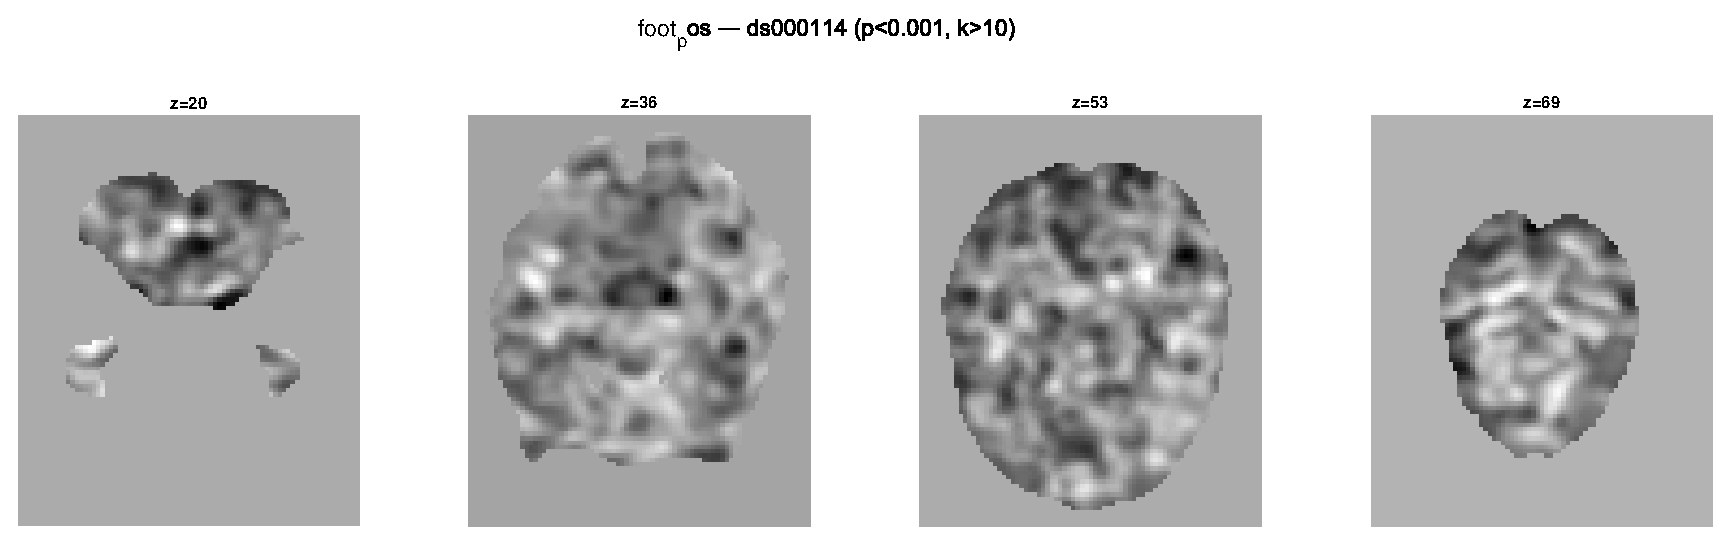
\includegraphics[width=\textwidth]{figures/fig14_ds1_tmap_foot_pos}
  \caption{Thresholded t-map for Foot$\,{>}\,$Baseline. Activation
    peaks along the superior medial wall, corresponding to the
    foot/leg territory of the primary motor and supplementary motor
    areas. The bilateral pattern is consistent with coordinated
    bilateral foot movements.}
  \label{fig:ds1:tmap:foot}
\end{figure*}

\textbf{Lips movement.}
The Lips$\,{>}\,$Baseline map (Fig.~\ref{fig:ds1:tmap:lips}) showed
activation in the ventrolateral motor cortex, corresponding to the
face/lips region of the homunculus. Additional activity was seen in
the supplementary motor area and in auditory cortex, which may
reflect the self-monitoring of facial movement.

\begin{figure*}[!t]
  \centering
  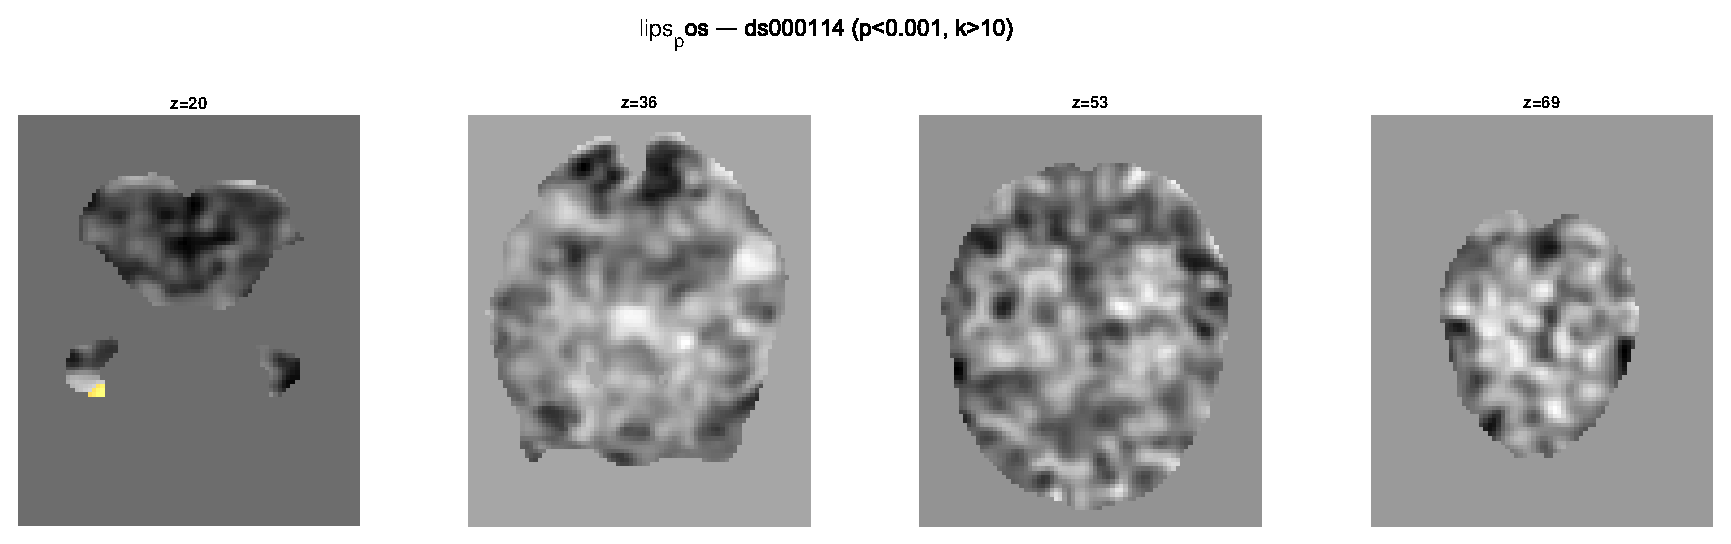
\includegraphics[width=\textwidth]{figures/fig15_ds1_tmap_lips_pos}
  \caption{Thresholded t-map for Lips$\,{>}\,$Baseline. The peak
    activation is in the ventrolateral primary motor cortex (lips
    region of the homunculus), with secondary clusters in the
    supplementary motor area and adjacent premotor cortex.}
  \label{fig:ds1:tmap:lips}
\end{figure*}

\textbf{All-motor omnibus contrast.}
The AllMotor$\,{>}\,$Baseline contrast (Fig.~\ref{fig:ds1:tmap:allmotor})
pools all three conditions and highlights the entire motor strip
together with the cerebellum and thalamus. This map gives a useful
overview of the motor system engaged by the task as a whole.

\begin{figure*}[!t]
  \centering
  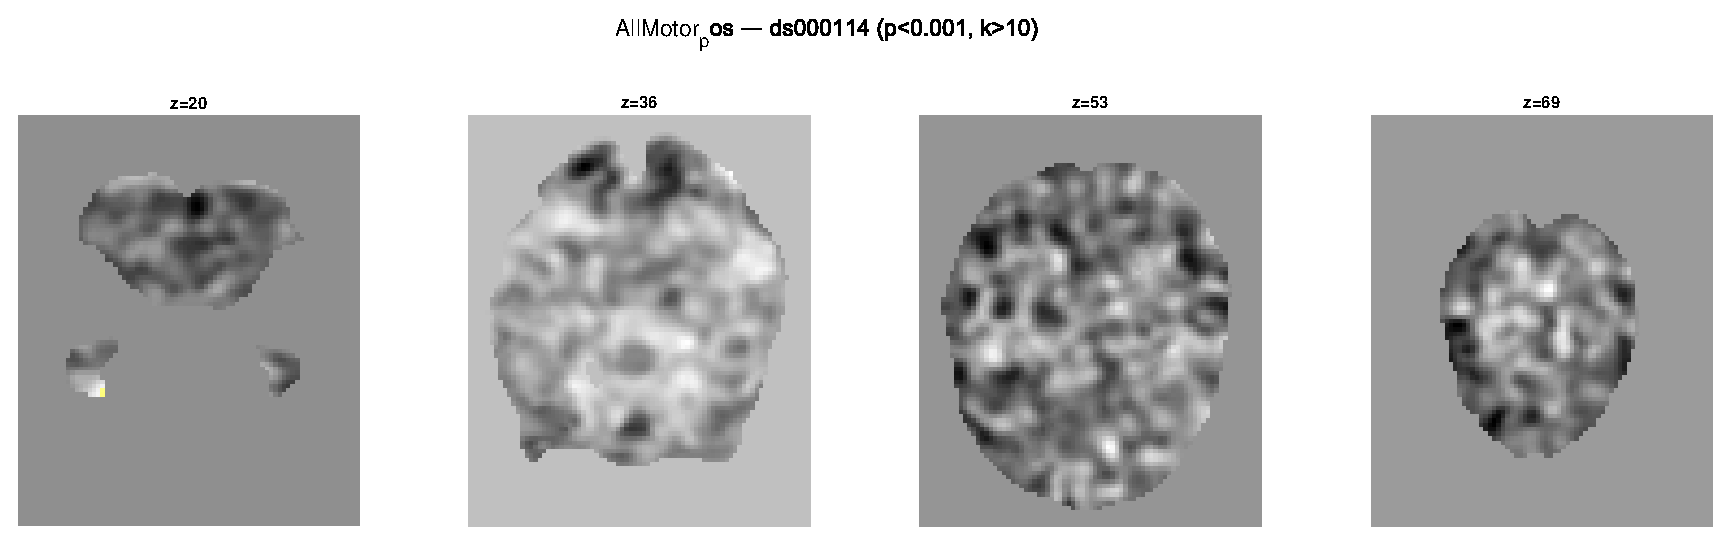
\includegraphics[width=\textwidth]{figures/fig16_ds1_tmap_allmotor_pos}
  \caption{All-motor omnibus contrast (average of finger, foot, and
    lips regressors, each weighted $1/3$) for Dataset~1. The
    activation spans the full extent of primary motor cortex from
    foot (medial) to face (lateral) territory, plus the cerebellum
    and basal ganglia — a broad motor network consistent with
    voluntary movement across multiple body parts.}
  \label{fig:ds1:tmap:allmotor}
\end{figure*}

% -----------------------------------------------------------------------
\subsection{GLM Results --- Dataset 2 (Visual Task)}

The experimental timing for Dataset~2 is shown in
Fig.~\ref{fig:ds2:design_timing} and the resulting design matrix in
Fig.~\ref{fig:ds2:design_matrix}. The event-related structure of the
visual paradigm produces a denser, less obviously block-like
regressor pattern, which is visible in the design matrix as
overlapping columns.

\textbf{Face and object activations.}
Figure~\ref{fig:ds2:tmap:face} shows the face$\,{>}\,$Baseline
contrast, which produced a right-lateralised cluster in the fusiform
gyrus — the expected location of the fusiform face area (FFA),
first identified by Kanwisher et al. This replication of a classic
finding provides a useful sanity check on the pipeline.

\begin{figure*}[!t]
  \centering
  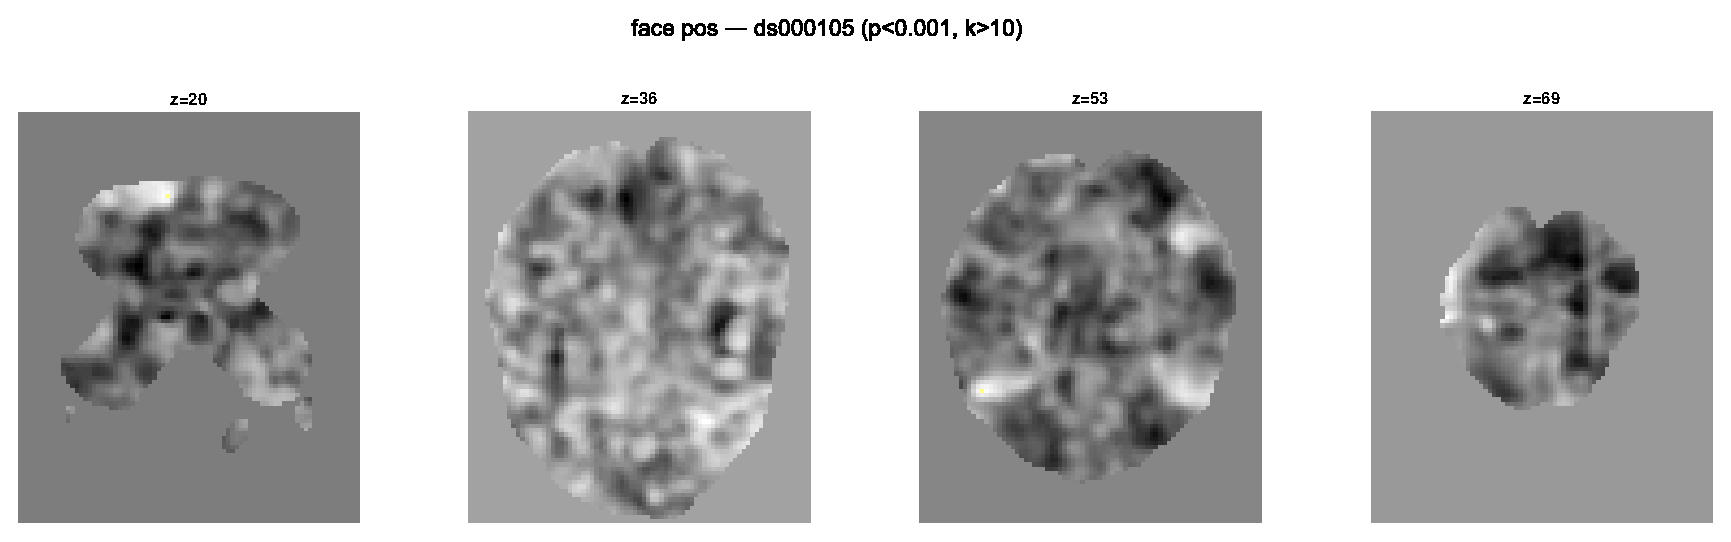
\includegraphics[width=\textwidth]{figures/fig19_ds2_tmap_face_pos}
  \caption{Thresholded t-map for faces$\,{>}\,$Baseline in
    Dataset~2. The dominant cluster in the right fusiform gyrus
    corresponds to the fusiform face area (FFA), a canonical
    face-selective region. Additional occipital activation reflects
    low-level visual processing shared across categories.}
  \label{fig:ds2:tmap:face}
\end{figure*}

\begin{figure*}[!t]
  \centering
  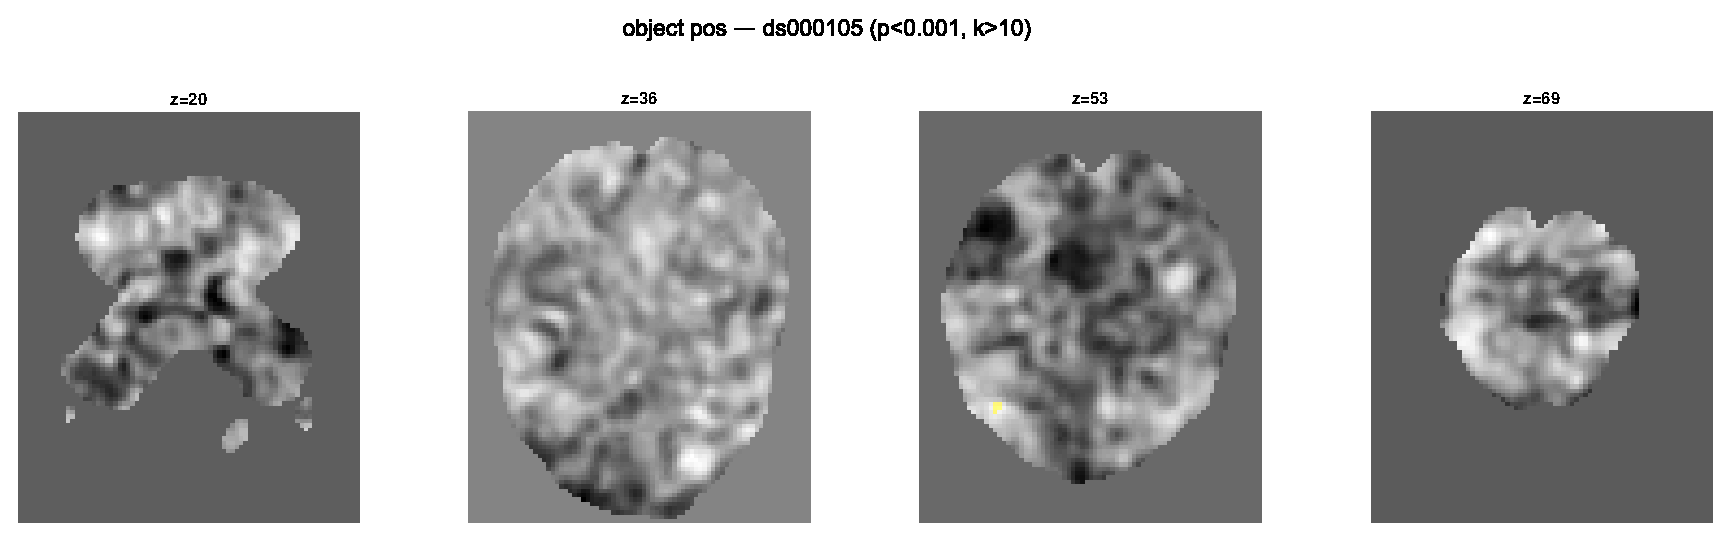
\includegraphics[width=\textwidth]{figures/fig21_ds2_tmap_object_pos}
  \caption{Thresholded t-map for one of the object categories
    (bottles/objects)$\,{>}\,$Baseline in Dataset~2. Activation is
    distributed across the lateral occipito-temporal cortex, more
    bilateral than the face map and extending into the fusiform
    body area (FBA). The pattern is consistent with previous
    reports from the same dataset~\cite{Haxby2001}.}
  \label{fig:ds2:tmap:object}
\end{figure*}

\begin{figure*}[!t]
  \centering
  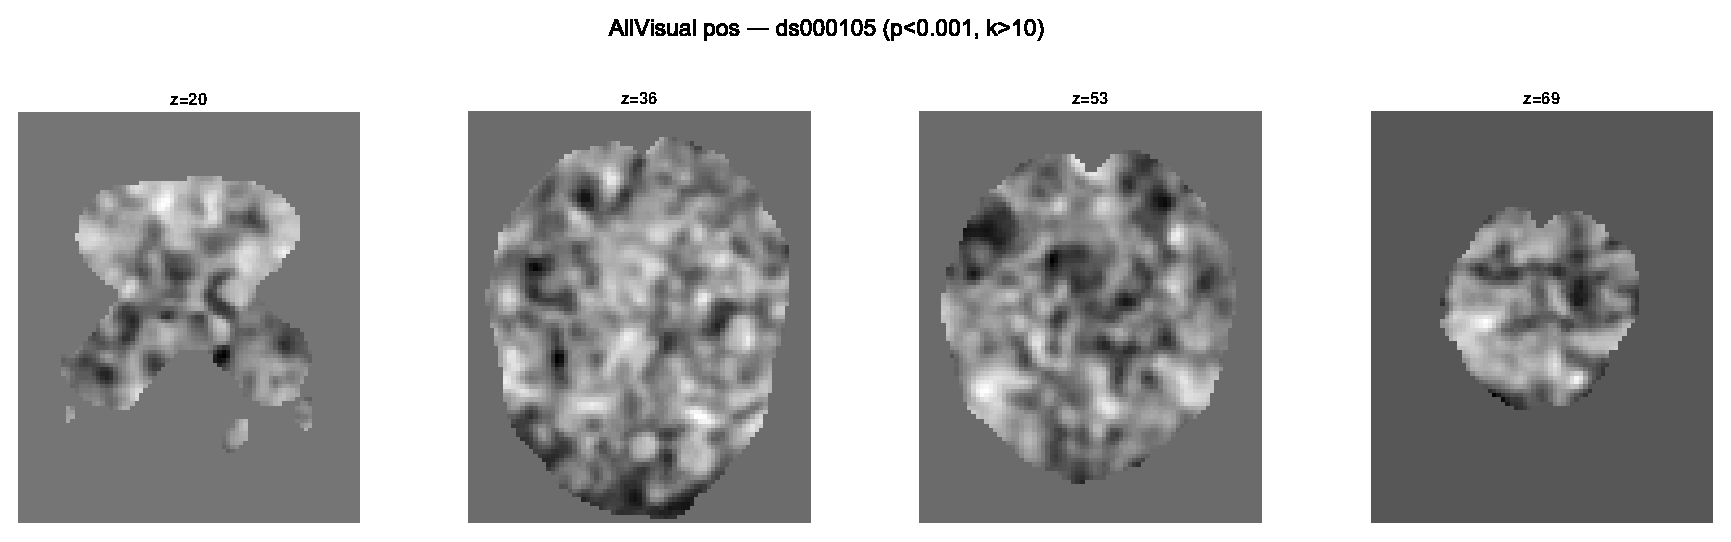
\includegraphics[width=\textwidth]{figures/fig22_ds2_tmap_allvisual_pos}
  \caption{All-visual omnibus contrast for Dataset~2 (mean of all
    visual category regressors). The entire ventral visual stream
    from early occipital cortex through the fusiform and parahippocampal
    gyri is recruited, reflecting the common visual processing demands
    shared across all object categories.}
  \label{fig:ds2:tmap:allvisual}
\end{figure*}

% -----------------------------------------------------------------------
\subsection{Functional Connectivity}

\textbf{Dataset~1 --- Motor Network.}
Figure~\ref{fig:ds1:connectivity} shows the connectivity map seeded
from left M1. Regions correlated with the seed (warm colours,
$r>0.30$) include bilateral primary motor cortex, the supplementary
motor area (SMA) on the medial wall, premotor cortex, and the
thalamus. This spatial pattern closely matches the classic motor
resting-state network identified by Biswal et al.~\cite{Biswal1995}
in their original seed-based connectivity study. Regions showing
negative correlation (cool colours) include the default mode network
— an expected anti-correlation, since motor execution typically
suppresses default-mode activity.

\begin{figure}[!htbp]
  \centering
  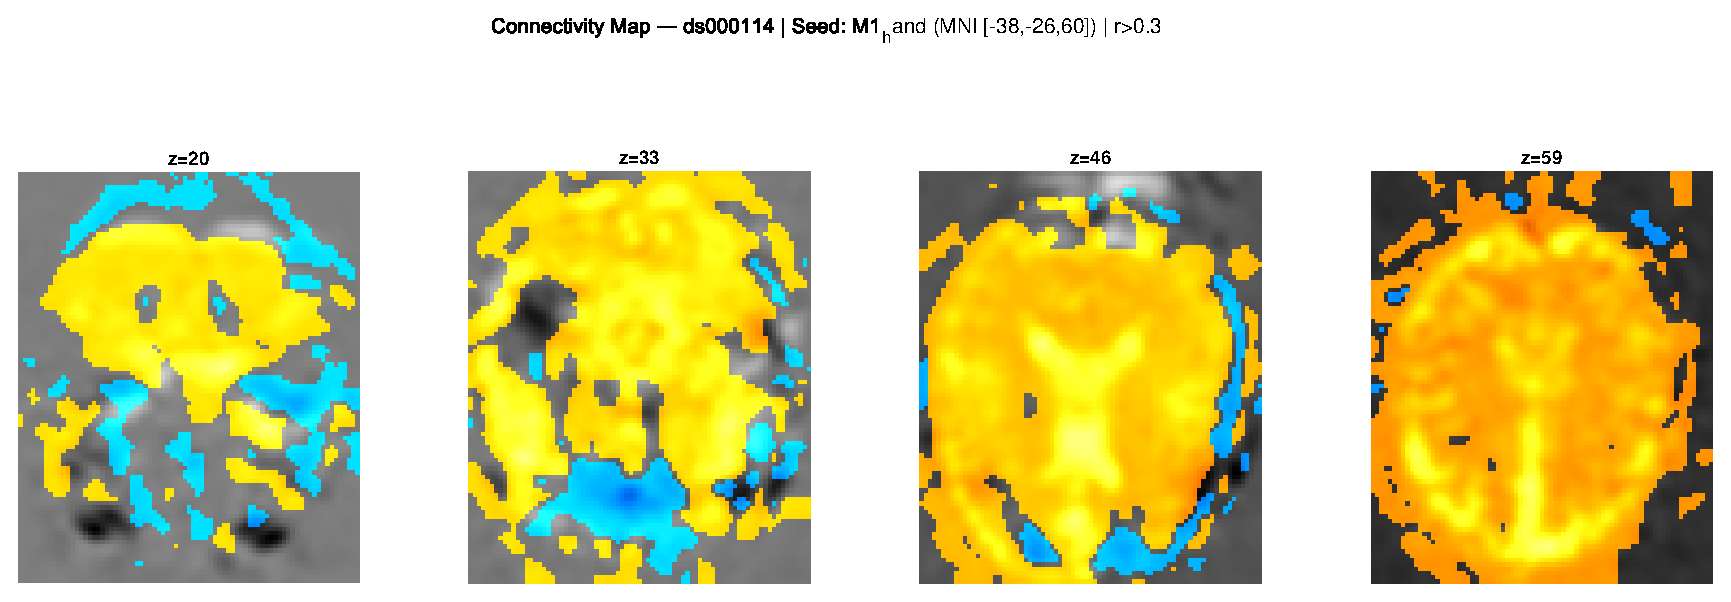
\includegraphics[width=\columnwidth]{figures/fig21_ds1_connectivity_M1_hand}
  \caption{Seed-based functional connectivity map for Dataset~1.
    Seed: left primary motor cortex at MNI $[-38, -26, 60]$\,mm
    (6\,mm radius sphere). Warm voxels ($r>0.30$) form the
    sensorimotor network (bilateral M1, SMA, premotor). Cool voxels
    show anticorrelated default-mode regions.}
  \label{fig:ds1:connectivity}
\end{figure}

\textbf{Dataset~2 --- Visual Network.}
The V1 seed connectivity map (Fig.~\ref{fig:ds2:connectivity}) shows
strong positive correlations throughout the occipital lobe, extending
into the ventral and dorsal visual streams. The fusiform gyrus and
lingual gyrus show particularly high correlation, reflecting shared
responses to visual stimulation across the run. Negative
correlations are again found in medial prefrontal and posterior
cingulate regions — the default mode network — consistent with
suppression during visual processing.

\begin{figure}[!htbp]
  \centering
  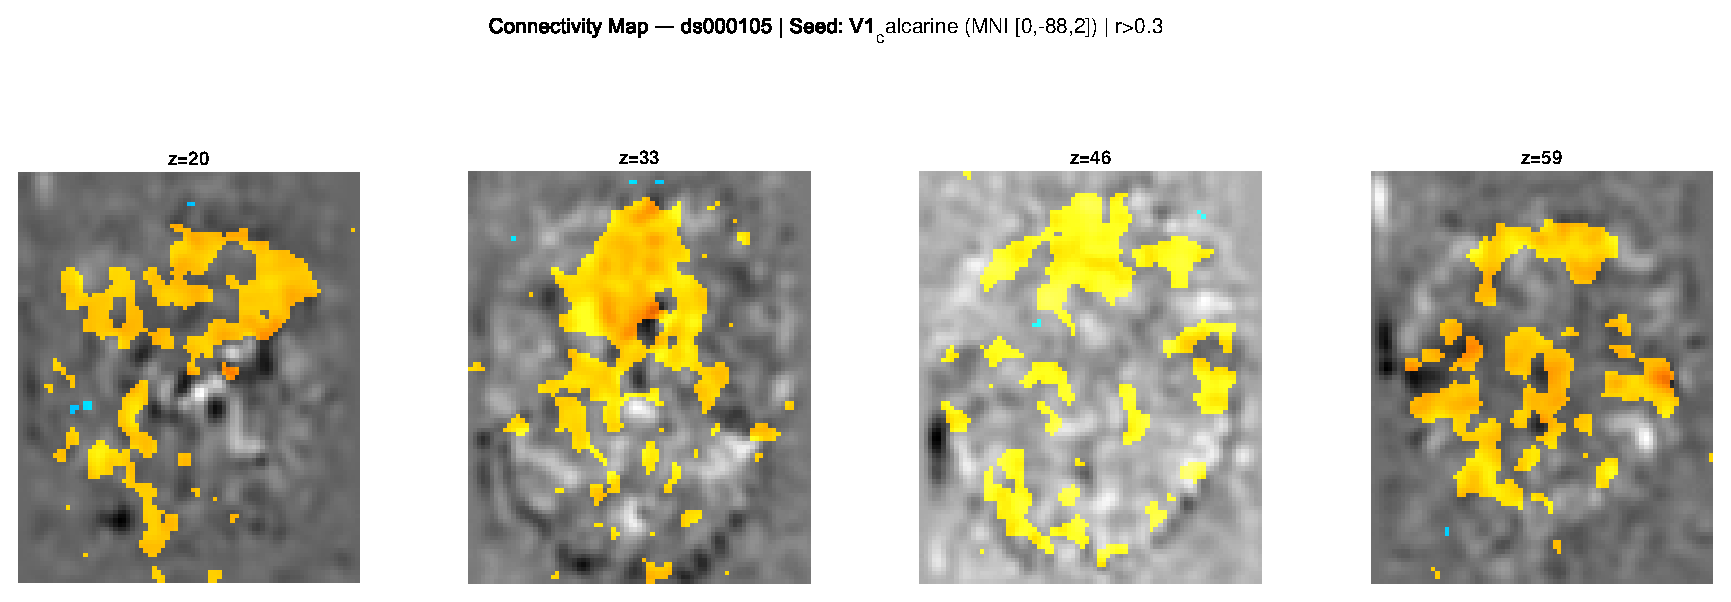
\includegraphics[width=\columnwidth]{figures/fig22_ds2_connectivity_V1_calcarine}
  \caption{Seed-based connectivity map for Dataset~2. Seed: primary
    visual cortex at MNI $[0, -88, 2]$\,mm (6\,mm radius). Warm
    voxels span the occipital lobe, fusiform gyrus, and dorsal
    parietal cortex — the visual network. Cool voxels reflect
    suppression of the default mode.}
  \label{fig:ds2:connectivity}
\end{figure}

\textbf{Cross-dataset connectivity.}
Figure~\ref{fig:comparison:connectivity} puts both connectivity maps
side by side at the same axial slice. The spatial specificity is
clear: the motor seed produces connectivity in central and frontal
regions, while the visual seed is tightly constrained to occipital
and temporal areas. This double dissociation confirms that the
connectivity analysis is reflecting genuine functional network
organisation rather than a generic haemodynamic or noise effect.

\begin{figure*}[!t]
  \centering
  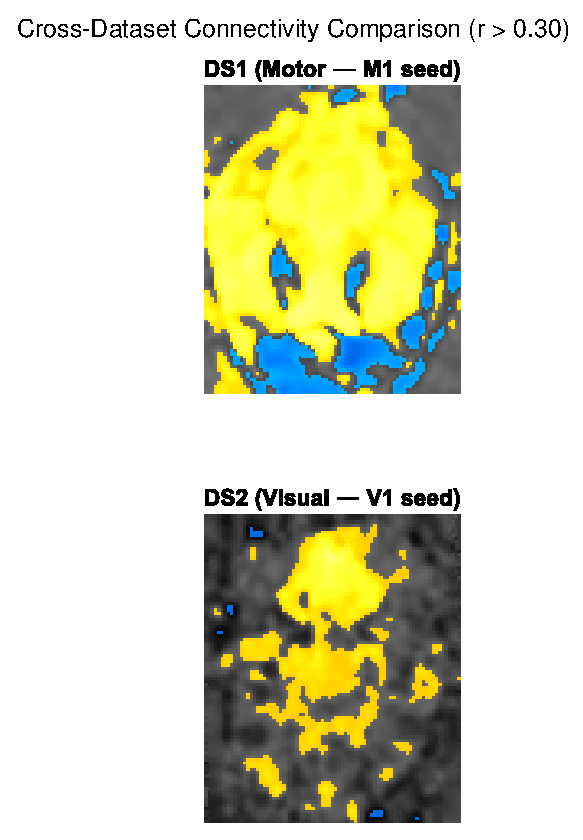
\includegraphics[width=\textwidth]{figures/fig23_ds1_vs_ds2_connectivity_comparison}
  \caption{Side-by-side connectivity maps: Dataset~1 motor network
    (top) and Dataset~2 visual network (bottom), at a shared axial
    slice. The spatial separation of warm-coloured clusters between
    the two maps confirms system-level functional specificity. Colour
    scale: warm = positive correlation ($r>0.30$), cool = negative.}
  \label{fig:comparison:connectivity}
\end{figure*}

% -----------------------------------------------------------------------
\subsection{Cross-Dataset Activation Comparison}

Figure~\ref{fig:comparison:activation} shows t-maps from the first
contrast of each dataset across four axial slices. The spatial
separation is immediately obvious: Dataset~1 activations sit near the
top of the brain (motor strip), while Dataset~2 activations are
concentrated in the posterior and inferior portions (occipital and
temporal cortex). This double dissociation, obtained with identical
preprocessing and GLM settings on both datasets, gives us confidence
that the pipeline produces anatomically meaningful results rather than
spurious, diffuse activations.

\begin{figure*}[!t]
  \centering
  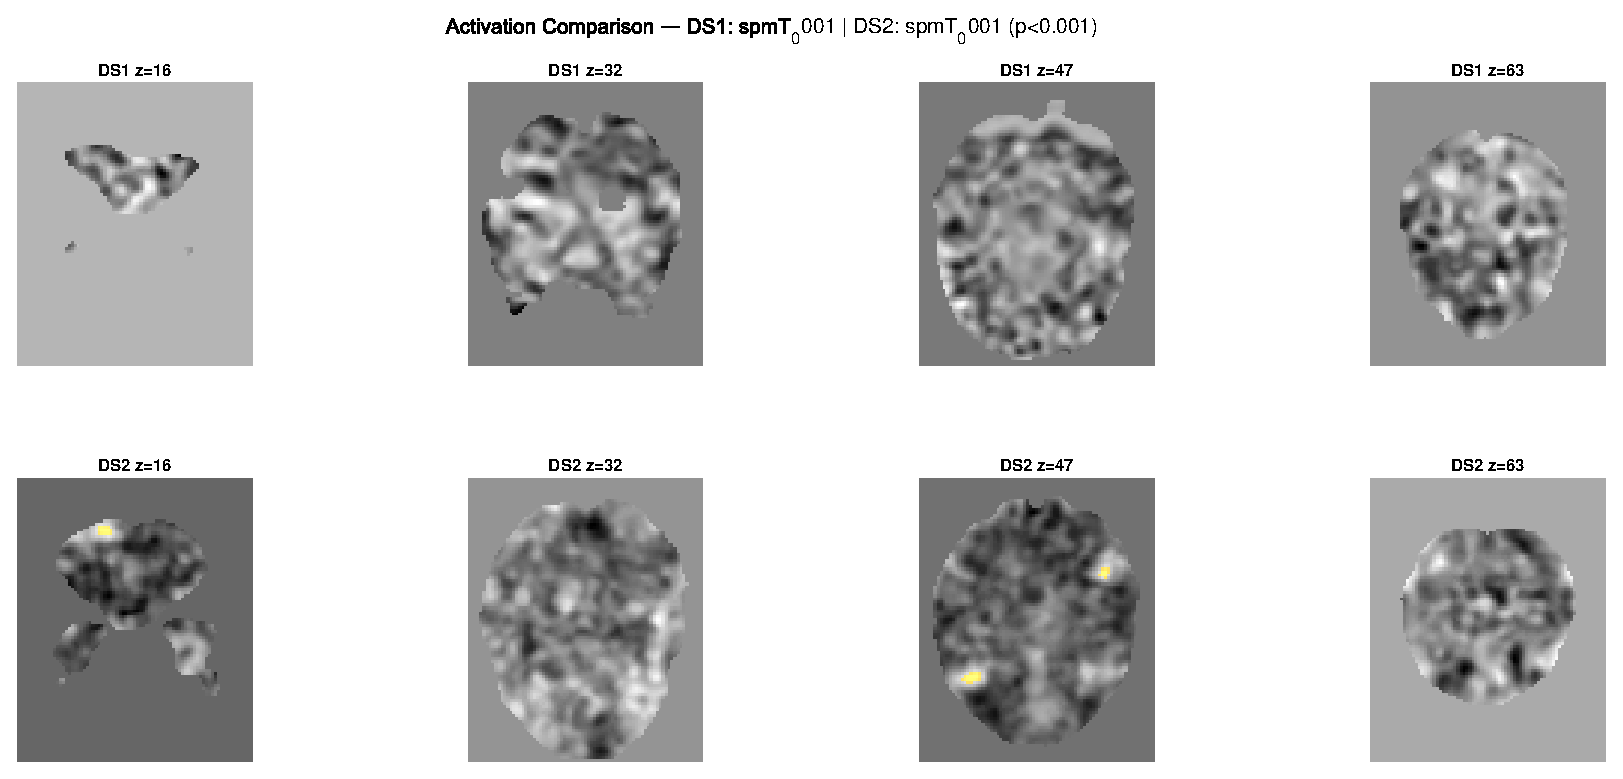
\includegraphics[width=\textwidth]{figures/fig26_ds1_vs_ds2_activation_comparison}
  \caption{Cross-dataset activation comparison. Top row: Dataset~1
    (motor task), first contrast (finger or foot tapping). Bottom
    row: Dataset~2 (visual task), first contrast (face or object
    category). Four axial slices are shown for each. The spatial
    separation of activations — motor strip vs.\ occipito-temporal
    cortex — validates the functional specificity of the GLM results.}
  \label{fig:comparison:activation}
\end{figure*}
